\documentclass[fontsize=11pt]{article}
\usepackage{amsmath}
\usepackage[utf8]{inputenc}
\usepackage[margin=0.75in]{geometry}
\usepackage{hyperref}
\hypersetup{
    colorlinks=true,
    linkcolor=blue,
    filecolor=magenta,      
    urlcolor=blue,
    pdftitle={Overleaf Example},
    pdfpagemode=FullScreen,
    }
\usepackage{graphicx}
\graphicspath{ {./images/} }
\urlstyle{same}
\title{CSC111 Project 2 Proposal: 

The Analysis of Summer Olympics Through External Effects 

(1940 - 2020)}
\author{Anh Dang Phuong, Dimitrios Gkiokmema, Dora Gombar, Maya Edri}
\date{\today}

\begin{document}
\maketitle

\section*{1., Problem Description and Research Question}

\textit{How did external - geopolitical, and societal - factors influence the outcomes and dynamics of the Olympic Games?}
\\
\\
Over the last 100 years, many historical occurrences have created tension while trying to perform in the Olympic Games, leaving an indelible mark on its history, fundamentally reshaping the competition landscape, and altering the trajectory of athletic achievement. 
\\
\\
Take, for instance, the impact of World Wars on the Olympics. Since the inception of the first modern Olympic Games in 1896, the sports game has faced cancellation on only three occasions: once during World War I (1916) and twice during World War II (1940, 1944). Yet, even in the post-war era, the scars of conflict lingered, leading to the decision to ban German and Japanese athletes from participating in 1948. 
\\ Afterward, during the Cold War, the Olympics became a battleground for ideological supremacy between the United States and the Soviet Union. The intense rivalry between the superpowers spilled onto the athletic stage, with each nation leveraging sporting success to bolster their respective political agendas. Following the Soviet invasion of Afghanistan, tensions between the United States and the Soviet Union escalated, leading to President Jimmy Carter's announcement of a boycott of the 1980 Moscow Summer Games by the United States. In response, the Soviet Union boycotted the 1984 Summer Olympics in Los Angeles.
\\ Finally, the fall of the Soviet Union in 1991 was a watershed moment in modern history, and its impact rippled across various facets of global affairs, including the Olympic competition. The Soviet Union formally dissolved and broke into fifteen separate nations, which altered the Olympic community's balance of power and presented logistical challenges as new nations tried to establish their sporting infrastructure.
\\
\\
The abovementioned examples - which are only fragments of the whole picture - perfectly illustrate the intricate background of the Olympic Games, indicating that sports results come not only from human capital but also from geopolitical and societal factors - often foreseen. Our project aims to emphasize, represent, and visualize such (international) historical events through the lens of our statistical computation approach: we plan to use graphical tree representations, pie and bar charts, and graphs.

\section*{2., Computational Plan}

TODO

 • Total medals in a given year

 • Total medals for a given country

 • Compare the number of Gold, Silver, and Bronze

 • Ranking (i.e. which country ranked the $i^{th}$ place for the number of (G/S/B/total) medals in year X?)

• Calculate the average duration of a country's success by measuring the number of consecutive editions in which a country wins medals. 

• Host Country Effect:
Analyze the impact of hosting the Olympics on a country's performance. Calculate the difference in medal counts for host countries in the year they hosted compared to non-host years.

• Team vs. Individual Sports Impact:
Analyze the impact of team sports versus individual sports on a country's overall medal count. Identify countries that excel in one category over the other.


\begin{figure}
    \centering
    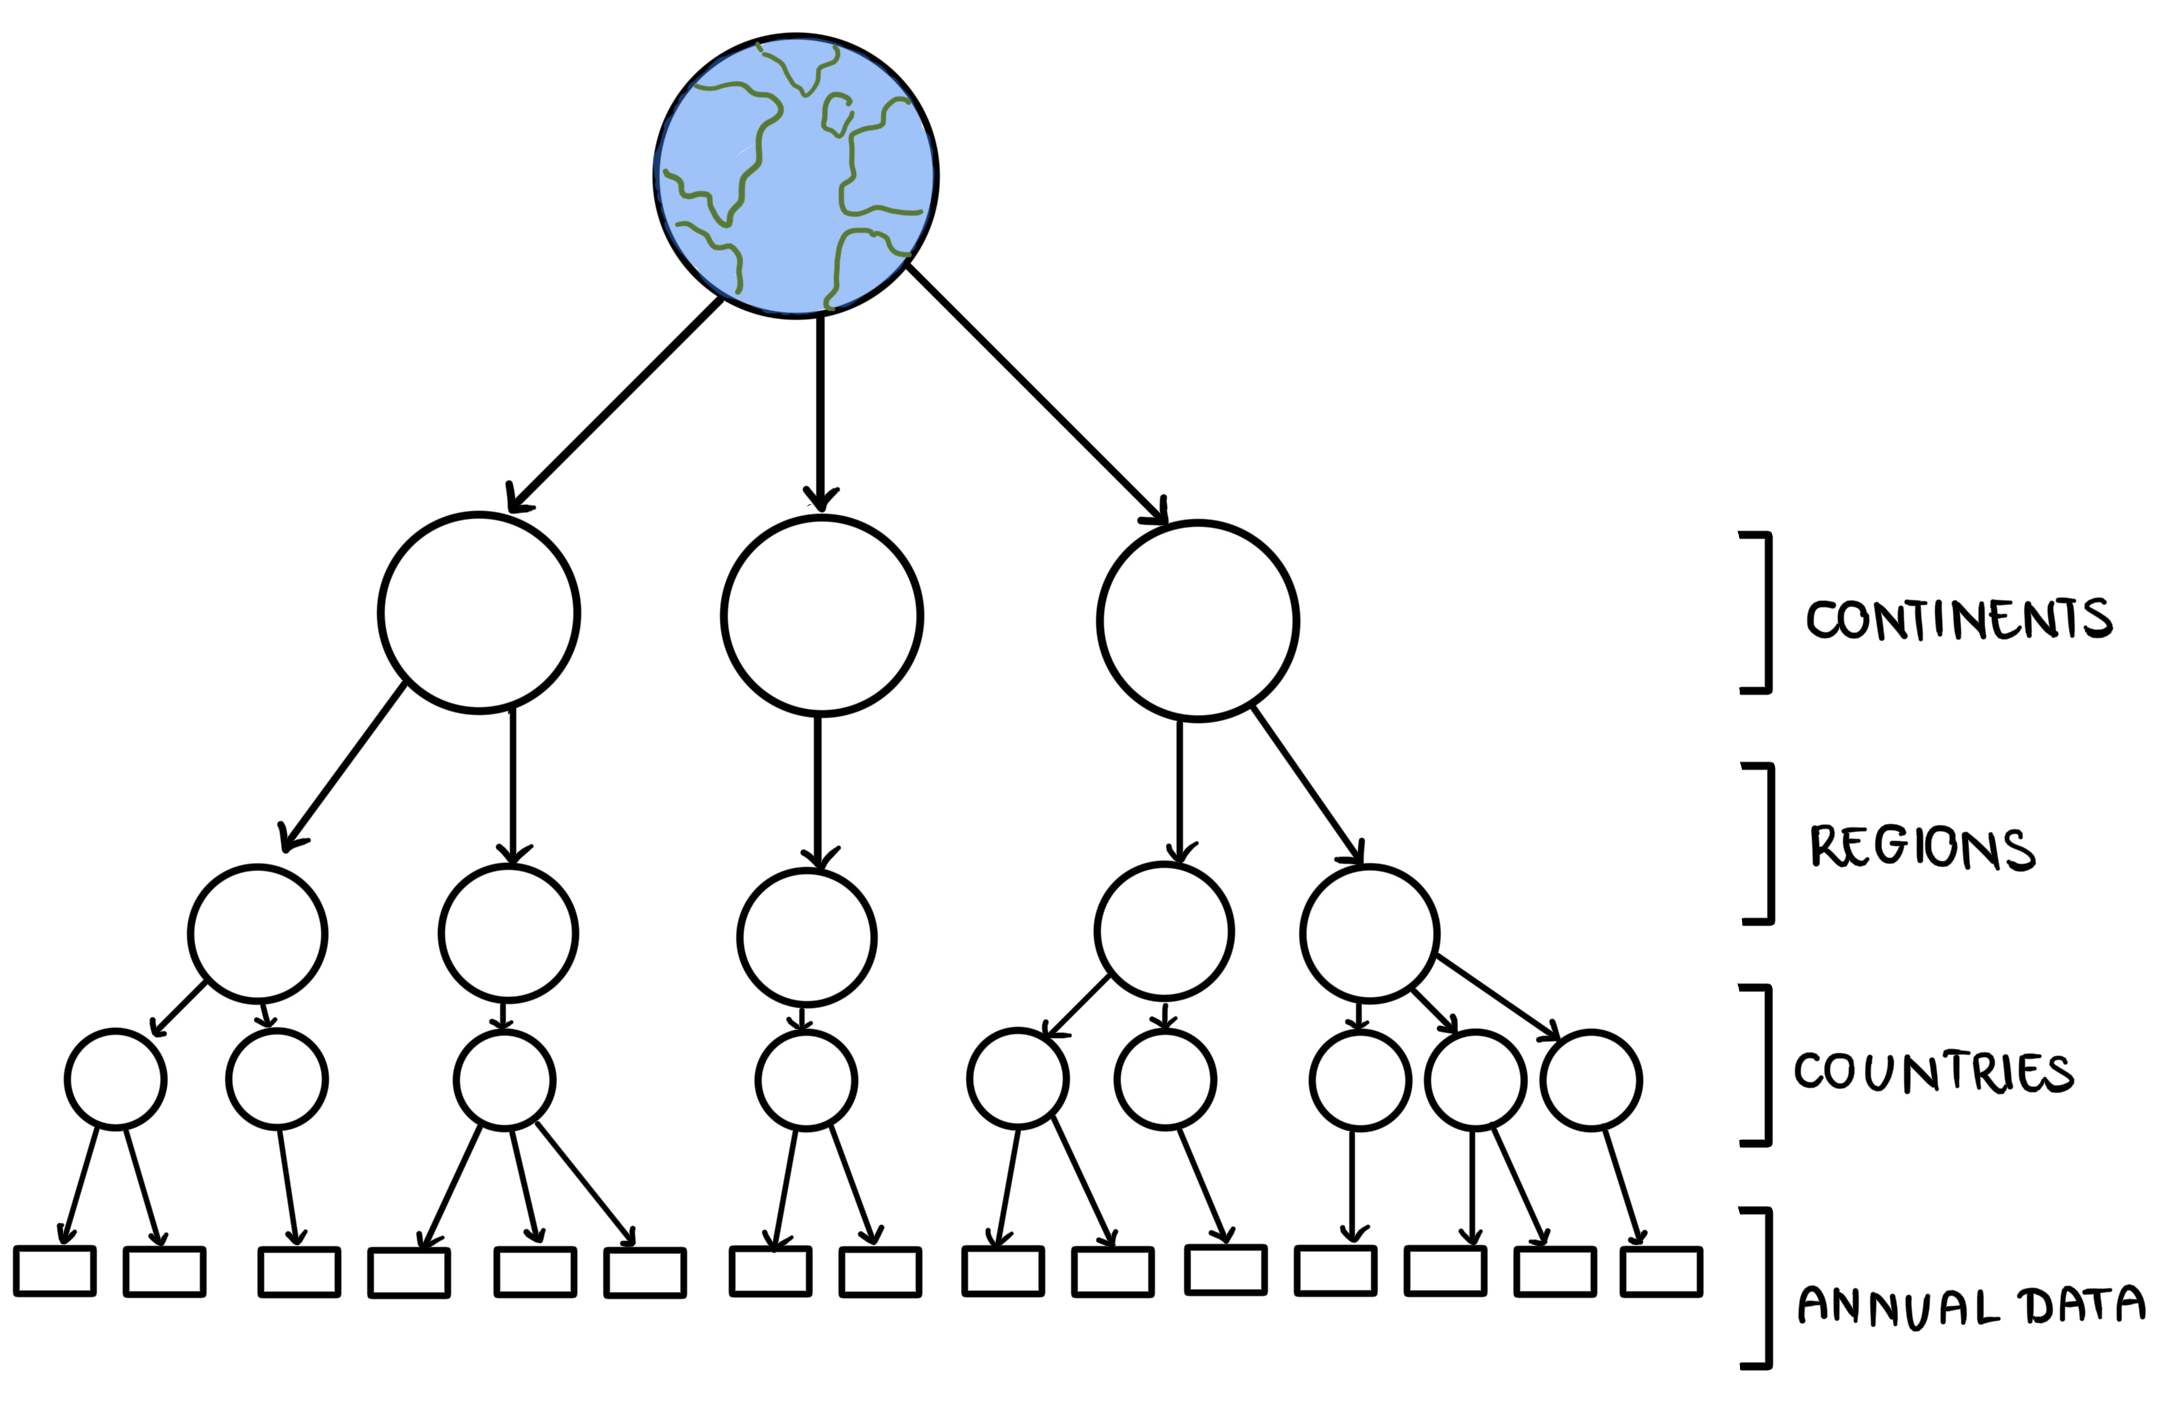
\includegraphics[width=0.5\linewidth]{tree_representation.jpg}
    \caption{Our representation of the Node-based Tree structure}
    \label{fig:enter-label}
\end{figure}

\section*{3., Computational Plan}

Our project will incorporate datasets on world population and outcomes of the Olympic games to show the interconnectedness of these factors. These datasets will be downloaded as csv files. The process of extracting (reading) the data from these files should not be too dissimilar to the txt files used in project one. All this data will be stored in a single tree, which will be the central part of our main. Methods we create will use the data stored in the tree to perform calculations, whose results will be displayed on graphs in PyGame. The hierarchy of the tree will be world, continents, continent sections (northern, eastern, central, etc.), countries, years. The years will be objects of the year class, which contain information about the type and number of medals won, players who participated in the games, where the game was held at that year, etc. The countries will be objects of the country dataset, which holds information about the games it hosted. We might make object classes for the other levels of the hierarchy later in the project, but currently we are thinking of simply writing the hierarchy's name in the tree's roots, for example: since continents don't have a class, the name of the continent will be a tree's root. Our code will utilize numerous datasets to provide a clear visualization of just how connected they are (population, Olympic games, and maybe some other data). One of these datasets has information on the games from 1896-2020. Here is its citation: 

  

“Summer Olympic Medals 1896 - 2020.” Www.kaggle.com, www.kaggle.com/datasets/ramontanoeiro/summer-olympic-medals-1986-2020. Accessed 28 Feb. 2024. 

  

This is a csv file, and an example of its data is: 1896, Greece, Athens, Great Britain, GBR, 2, 3, 2 

  

One computation we will perform (after creating the tree from the datasets) is to see if host countries win more often by counting the number of games won by the host country and seeing if this is greater than the total number of games held. Another calculation we will do is to find if historical events (wars, stock market crash, etc.) had an impact on the Olympics. We will measure the impact by calculating the standard deviation of the medals given at the Olympic games each year, and seeing if the number of medals lies far away from the mean. An outlier is a data point that is “three standard deviations from the mean may be considered an outlier” (Peter K Dunn, Scientific Research and Methodology) 

Dunn, Peter K. Scientific Research Methods. Bookdown.org, bookdown.org/pkaldunn/Book/. 

If such outliers coincide with historical events, our hypothesis is proven correct. Lastly, our results will be displayed on graphs drawn in PyGame. The graphs will clearly show the interaction of population and historical events on the Olympic games.

\section*{4., References}

\begin{enumerate}
    \item Carter, Jimmy. 1995. \textit{Keeping Faith: Memoirs of a President}. University of Arkansas pbk. ed. Fayetteville, AR: University of Arkansas Press.
    \item Grannan, Cydney. 2016. “7 Significant Political Events at the Olympic Games | Britannica.” Encyclopedia Britannica. July 29, 2016.  \url{https://www.britannica.com/list/7-significant-political-events-at-the-olympic-games}.
    \item International Organization on Standardization. 1999. “UNSD — Methodology.” United Nations: Statistics Division. 1999. \url{https://unstats.un.org/unsd/methodology/m49/}.
    \item IOC Research and Reference Service. 2017. “Olympic Sports and Medals, 1896-2014.” Kaggle. 2017. \url{https://www.kaggle.com/datasets/the-guardian/olympic-games?select=summer.csv}.
    \item Johnston, Mindy. 2024. “Moscow 1980 Olympic Games | Boycott, Cold War, USSR, \& Summer Games | Britannica.” Encyclopedia Britannica. February 28, 2024. \url{https://www.britannica.com/event/Moscow-1980-Olympic-Games}.
    \item Miller, David. 2012. \textit{The Official History of the Olympic Games and the IOC: Athens to London}, 1894-2012. Edinburgh: Mainstream Pub.
    \item Ritchie, Hannah, Lucas Rodés-Guirao, Edouard Mathieu, Marcel Gerber, Esteban Ortiz-Ospina, Joe Hasell, and Max Roser. 2023. “Data Page: Population.” Our World in Data. 2023. \url{https://ourworldindata.org/grapher/population}.
\end{enumerate}

\end{document}
